\subsection{Vòng lặp while}
\label{while}
Sử dụng vòng lặp while để lặp đi lặp loại một khối lệnh khi số lần lặp phụ thuộc vào điều kiện lặp. Cấu trúc của vòng lặp while:\par
\texttt{while <condition>:}\par
\qquad \texttt{//while block's code}\par
\texttt{[else:}\par
\qquad \texttt{//else block's code]}\par
\begin{figure}[h]
	\centering
	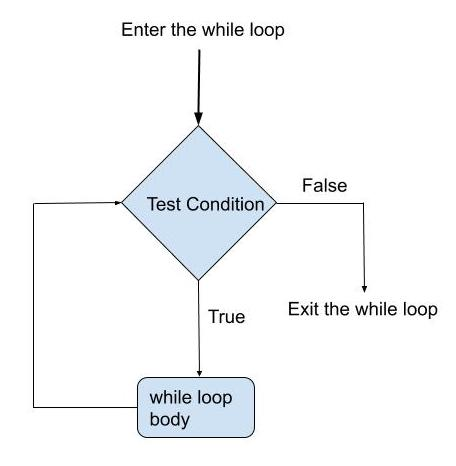
\includegraphics[width=0.5\linewidth]{img/while}
	\caption{Mô tả cách thức hoạt động của vòng lặp while}
	\label{fig:while}
\end{figure}
\newpage
\textbf{Ví dụ:} Chương trình nhập vào một số, in ra các bội nhỏ hơn 100 của số đó :\\
\rule{\linewidth}{0.2mm}\par
\begin{linenumbers}
	\texttt{n = \textcolor{red}{int}(\textcolor{blue}{input}("Type a number: "))}\par
	\texttt{multiple = n}\par
	\texttt{i = 2}\par
	\texttt{\textcolor{red}{while} multiple < 100:}\par
	\qquad \texttt{\textcolor{blue}{print}(multiple)}\par
	\qquad\texttt{multiple = n}\par
	\qquad\texttt{multiple *= i}\par
	\qquad\texttt{i += 1}\par
\end{linenumbers}
\rule{\linewidth}{0.2mm}\par
\noindent
\resetlinenumber
Kết quả cho ra ở Console:\\
\rule{\linewidth}{0.2mm}\par
\begin{linenumbers}
	\texttt{Type a number: 28}\par
	\texttt{28}\par
	\texttt{56}\par
	\texttt{84}\par
\end{linenumbers}
\rule{\linewidth}{0.2mm}\par
\resetlinenumber
\newpage
\textbf{Ví dụ:} Chương trình nhập vào hai số tự nhiên, tính ước chung lớn nhất của hai số đó:\\
\rule{\linewidth}{0.2mm}\par
\begin{linenumbers}
	\texttt{\textcolor{blue}{print}("GCD(a, b)")}\par
	\texttt{\textcolor{blue}{print}("a must be greater than b")}\par
	\texttt{a = \textcolor{red}{int}(\textcolor{blue}{input}("a = "))}\par
	\texttt{b = \textcolor{red}{int}(\textcolor{blue}{input}("b = "))}\par
	\texttt{\textcolor{red}{while} a \% b != 0:}\par
	\qquad \texttt{temp = a}\par
	\qquad \texttt{a = b}\par
	\qquad \texttt{b = temp \% b}\par
	\texttt{\textcolor{red}{else}:}\par
	\qquad\texttt{\textcolor{blue}{print}("GCD:", b)}\par
\end{linenumbers}
\rule{\linewidth}{0.2mm}\par
\noindent
\resetlinenumber
Kết quả cho ra ở Console:\\
\rule{\linewidth}{0.2mm}\par
\begin{linenumbers}
	\texttt{GCD(a, b)}\par
	\texttt{a must be greater than b}\par
	\texttt{a = 126}\par
	\texttt{b = 12}\par
	\texttt{GCD: 6}\par
\end{linenumbers}
\rule{\linewidth}{0.2mm}\par
\resetlinenumber
\newpage
\textbf{Ví dụ:} Chương trình nhập vào số thập phân, in ra màn hình số nhị phân của số đó:\\
\rule{\linewidth}{0.2mm}\par
\begin{linenumbers}
	\texttt{n = \textcolor{red}{int}(\textcolor{blue}{input}("Type your decimal number: "))}\par
	\texttt{binary = ""}\par
	\texttt{\textcolor{red}{while} n > 0:}\par
	\qquad \texttt{binary += "\%s" \% (n \% 2) \# convert surplus of n / 2 to string and add to binary	
	}\par
	\qquad \texttt{n = int(n / 2)}\par
	\texttt{\textcolor{blue}{print}("Binary:", binary[::-1]) \# reverse binary string}\par
\end{linenumbers}
\rule{\linewidth}{0.2mm}\par
\noindent
\resetlinenumber
Kết quả cho ra ở Console:\\
\rule{\linewidth}{0.2mm}\par
\begin{linenumbers}
	\texttt{Type your decimal number: 13}\par
	\texttt{Binary: 1101}\par
\end{linenumbers}
\rule{\linewidth}{0.2mm}\par
\resetlinenumber
\newpage